\documentclass[aps,letterpaper,10pt]{revtex4}

\usepackage{graphicx} % For images
\usepackage{float}    % For tables and other floats
\usepackage{verbatim} % For comments and other
\usepackage{amsmath}  % For math
\usepackage{amssymb}  % For more math
\usepackage{fullpage} % Set margins and place page numbers at bottom center
\usepackage{listings} % For source code
\usepackage{subfig}   % For subfigures
\usepackage[usenames,dvipsnames]{color} % For colors and names
\usepackage[pdftex]{hyperref}           % For hyperlinks and indexing the PDF
\hypersetup{ % play with the different link colors here
    colorlinks,
    citecolor=blue,
    filecolor=blue,
    linkcolor=blue,
    urlcolor=blue % set to black to prevent printing blue links
}

\definecolor{mygrey}{gray}{.96} % Light Grey
\lstset{
	language=[ISO]C++,              % choose the language of the code ("language=Verilog" is popular as well)
   tabsize=3,							  % sets the size of the tabs in spaces (1 Tab is replaced with 3 spaces)
	basicstyle=\tiny,               % the size of the fonts that are used for the code
	numbers=left,                   % where to put the line-numbers
	numberstyle=\tiny,              % the size of the fonts that are used for the line-numbers
	stepnumber=2,                   % the step between two line-numbers. If it's 1 each line will be numbered
	numbersep=5pt,                  % how far the line-numbers are from the code
	backgroundcolor=\color{mygrey}, % choose the background color. You must add \usepackage{color}
	%showspaces=false,              % show spaces adding particular underscores
	%showstringspaces=false,        % underline spaces within strings
	%showtabs=false,                % show tabs within strings adding particular underscores
	frame=single,	                 % adds a frame around the code
	tabsize=3,	                    % sets default tabsize to 2 spaces
	captionpos=b,                   % sets the caption-position to bottom
	breaklines=true,                % sets automatic line breaking
	breakatwhitespace=false,        % sets if automatic breaks should only happen at whitespace
	%escapeinside={\%*}{*)},        % if you want to add a comment within your code
	commentstyle=\color{BrickRed}   % sets the comment style
}

\newcommand{\labno}{05}
\newcommand{\labtitle}{AU 332 Artificial Intelligence: Principles and Techniques}
\newcommand{\authorname}{Guowei Deng}
\newcommand{\professor}{Yue Gao}

\begin{document}

\begin{titlepage}
\begin{center}
{\Large \textsc{\labtitle} \\ \vspace{4pt}}
\rule[13pt]{\textwidth}{1pt} \\ \vspace{150pt}
{\large By: \authorname \\ \vspace{10pt}
Instructor: \professor \\ \vspace{10pt}
\today}

\end{center}
\end{titlepage}
\section{Question 1}
The question 1 is quite simple. Just change the return value to ``a+b''.\\
\section{Question 2}
To solve the question 2, we need find the function \emph{buyLotsOfFruit}. I use a for loop to get the imformation in \emph{orderList} and calculate the totalCost using the code\\
\lstinputlisting{code.c}
	\vspace{3mm}
\section{Question 3}
To solve the question 3, first we need to understand the code in anther document \emph{shop.py}.In \emph{shop.py}, a class \emph{FruitShop} is defined.Some related functions are defined as well. Among these functions, the function \emph{getPriceOfOrder} is useful for this function.\\
So function \emph{shopSmart} in \emph{shopSmart.py} should be implemented as follows.\\
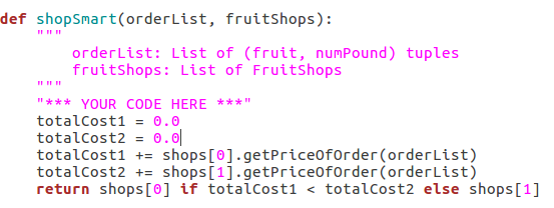
\includegraphics{question3.png}
\\First we define 2 variables to process the total cost in different shops. And then find the lowest value. After that, the function return the corresponding shop.\\
\section{Screenshot}
Here is the screenshot for these questions.\\
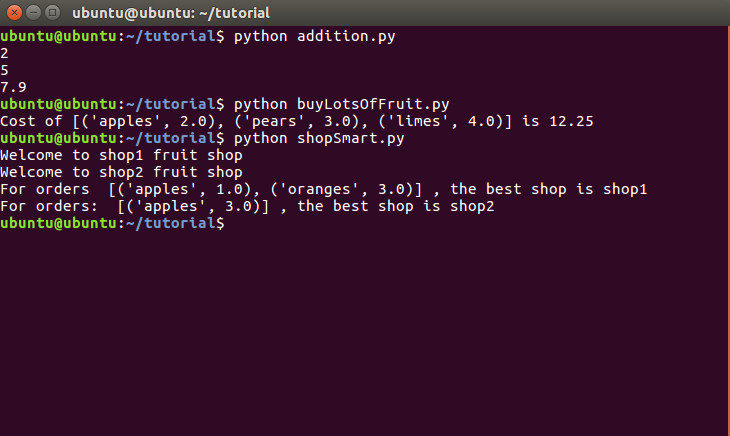
\includegraphics[scale=0.8]{Screenshot.png}
\end{document}

